\chapter[Metodologia]{Metodologia}
Neste capítulo é apresentado como foi realizada a implementação do algoritmo de treinamento do classificador LDA em um sistema coprocessado hardware-software, detalhando todos os módulos que compõem a implementação.

\section{Algoritmo Implementado}
Em 2010 o francês Fabien Lotte publicou um trabalho com objetivo de comparar as implementações de algoritmos de extração de características de sinais provenientes de atividades cerebrais, além de propor um novo algoritmo para extração de características dos sinais \cite{F.Lotte}.\\
Para coleta de resultados Lotte utilizou o algoritmo de classificação LDA e a base de dados \textit{BCI Competition III - Dataset IVa} obtendo como melhor resultado o extrator de características CSP, conforme apresentado anteriormente na Tabela \ref{arte_state}.\\
O algoritmo foi desenvolvido utilizando a plataforma \textit{Matlab}, onde foram utilizados os recursos e funções da plataforma. A Figura \ref{processos_alg} apresenta um diagrama de processo que descreve as funções utilizadas no algoritmo.

\begin{figure}[h]
	\centering
	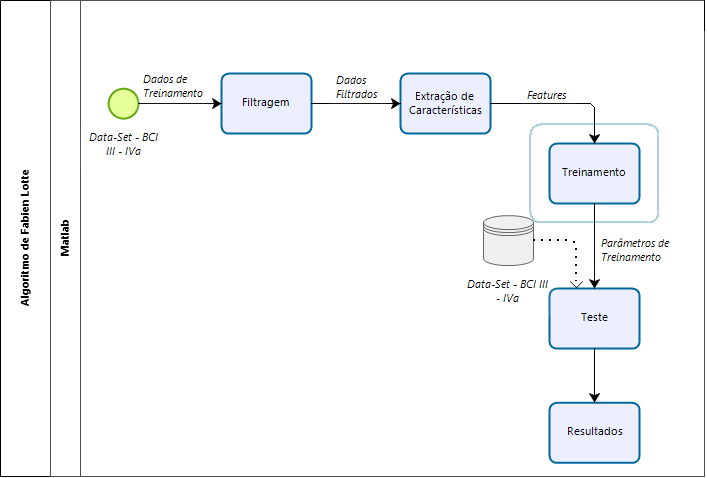
\includegraphics[keepaspectratio=true,scale=0.6]{figuras/Processos_Algoritmo_Lotte.PNG}
	\caption{Processos realizados pelo algoritmo de \cite{F.Lotte}.}
	\label{processos_alg}
\end{figure}

Utilizando-se dos dados de treinamento do \textit{Data set - BCI Competition III - IVa}, o algoritmo inicia-se realizando a filtragem do sinal, a partir de um filtro \textit{Butterworth} de {$5^a$} ordem, mantendo os sinais das faixas {$\alpha$} e {$\beta$}, e atenuando as demais frequências. Em seguida, é realizado o processo de extração de características utilizando o algoritmo CSP. Logo após, é realizado o processo de treinamento, onde são calculados hiperplanos que melhor separam as classes. Por fim, para o processo de teste são atribuídos os sinais de teste, também fornecidos pelo \textit{Data Set - BCI Competition III -IVa}e os hiperplanos calculados no processo de treinamento, seguido da disponibilização dos resultados de acurácia e tempo de treinamento.

\section{Implementação em Sistema Coprocessado}

Conforme apresentado, o objetivo deste trabalho é o estudo dos ganhos ou perdas no processamento do algoritmo de treinamento do classificador LDA implementado em um coprocessamento hardware-software, utilizando-se da plataforma \textit{Zynq} da placa \textit{Xilinx Zybo Board}, quando comparado com a implementação realizada por \cite{F.Lotte} e a implementação apenas em software utilizando o processador ARM.\\
Sendo assim, o trabalho se restringiu a implementação em sistema coprocessado o processo de treinamento (processo destacado) da Figura \ref{processos_alg}.\\
A Figura \ref{processos_train} apresenta um diagrama de processos que descreve a função de treinamento do classificador LDA.

\begin{figure}[h]
	\centering
	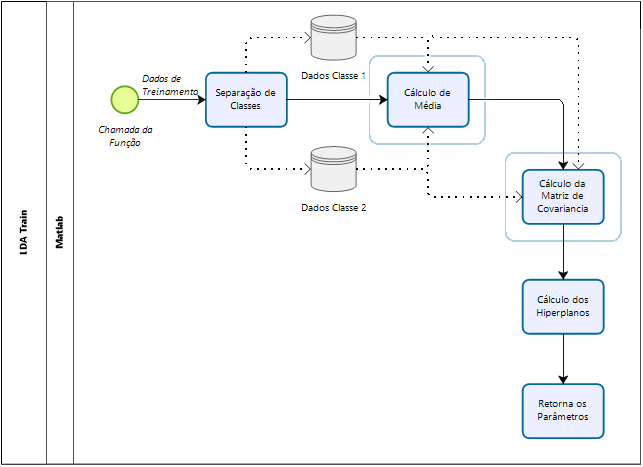
\includegraphics[keepaspectratio=true,scale=0.6]{figuras/Processos_LDA_Train.PNG}
	\caption{Processos realizados pelo algoritmo de treinamento de um classificador LDA.}
	\label{processos_train}
\end{figure}

Inicialmente é realizada a separação dos sinais em dois conjuntos de dados que representam os dados referentes às duas classes em estudo. Em seguida são calculadas as médias dos sinais de cada classe. Este valor é repassado para a função de cálculo da matriz de covariância (ou correlação), onde são realizados cálculos matriciais conforme apresentado na Equação \ref{label}. Em seguida são calculados os hiperplanos a partir da correlação das características dos sinais. Estes hiperplanos representam os parâmetros de treinamento do classificador. São a partir deles que os sinais de teste são classificados.\\

Na realização do coprocessamento as funções de cálculo de média e cálculo de covariancia são as duas funções que apresentam um maior esforço computacional. Portanto ambas as funções foram mapeadas em hardware, utilizando-se da linguagem VHDL, a fim de acelerar o processamento utilizando o processamento paralelo em FPGA, enquanto as demais funções foram compiladas em software na linguagem C, executada através de um SO Linux embarcado nos processadores ARM.

\subsection{Dispositivos e ferramentas}
O algoritmo de treinamento do classificador LDA será implementado nas lógicas digitais da FPGA na plataforma Zynq da placa \textit{Zybo-Board}, utilizando \textit{IP-Cores} de cálculo aritmético em ponto flutuante, que são blocos matemáticos desenvolvidos com propriedades intelectuais \cite{munoz2010tradeoff} em unidade de ponto flutuante desenvolvidos por \cite{munoz2010tradeoff} e a linguagem descrição de hardware VHDL, a fim de paralelizar os processos do algoritmo. Para o mapeamento do algoritmo em VHDL será utilizado a plataforma \textit{Vivado}, que possui todas as ferramentas necessárias para descrição, simulação, síntese e implementação para FPGAs da \textit{Xilinx} \cite{zynqBook}.

\subsection{Metodologias de desenvolvimento}
Para implementação do algoritmo de treinamento do classificador LDA em FPGA será adotada a metodologia \textit{bottom-up}, na qual cada sub-bloco desenvolvido é testado antes de ser inserido ao bloco principal, bloco de integração de todos sub-blocos do projeto, também conhecido como \textit{Top module}.
Após a implementação e simulação do \textit{Top module}, será utilizado para teste e validação do hardware
 o \textit{dataset IVa} do \textit{BCI Competition III}, além de uma análise estatística do erro apresentado
usando como modelo de referência a implementação na plataforma \textit{Matlab} por \cite{F.Lotte}.

Para validação da eficiência do SoC serão coletados os dados das seguintes características:
\begin{itemize}
  \item Consumo de hardware: LUTs, FFs, blocos de DSP, blocos de memória RAM, I/O, MUX;
  \item Dados de desempenho: frequência de operação e tempo de execução;
  \item Estimação do consumo de energético.
  \item Estimação estatístico do erro de implementação.
\end{itemize}

Os processos de implementação do hardware em um SoC é apresentado na Figura \ref{diagram_hardware}.

\begin{figure}[h]
  \centering
  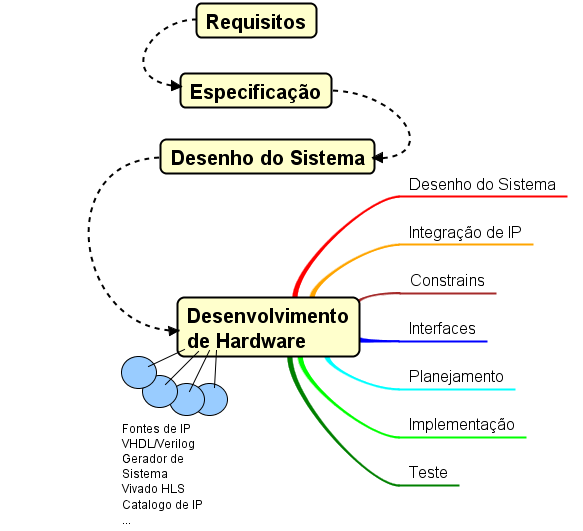
\includegraphics[keepaspectratio=true,scale=1.0]{figuras/fluxograma_hardware.PNG}
  \caption{Fluxograma de implementação de hardware em um SoC. Adaptado de \cite{zynqBook}}
  \label{diagram_hardware}
\end{figure}

\section{Implementação em software}
A seguir são apresentados os materiais, métodos e técnicas para a implementação do
algoritmo de treinamento do classificador LDA em software.

\subsection{Materiais}

Dispondo do SoC embarcado no kit de desenvolvimento da \textit{Zybo} (Digilent) , a implementação do algoritmo em 
software, explorará o processador \textit{ARM  Cortex -A9} de dois núcleos no \textit{Xilinx Zynq -7000}, usando também
o auxílio do sistema operacional \textit{Xilinux}. A codificação do algoritmo será feita na linguagem de programação \textit{C++}.

\subsection{Métodos e Técnicas}
 
Para o auxílio desta implementação, será instalado o sistema operacional \textit{Xilinux}, cujo os recursos e passos necessários
para a instalação do SO estão contidos em \cite{zynqBook}.
O processo para implementação seguirá o método \textit{bottom-up}, blocos de códigos menores serão implementados e testados
separadamente, com a finalização de todos os blocos serem integrados e testado em um único bloco principal. As entradas
para programa desenvolvido são provenientes do \textit{dataset IVa} do \textit{BCI Competition III}.

 
Os dados para análise após a implementação e teste serão:
\begin{itemize}[noitemsep]
\item Consumo de memória
\item Tempo de execução
\item Consumo de potência
\item Erro da implementação em comparação aos resultados obtidos por \cite{F.Lotte}
\end{itemize}

\section{\textit{Data Set IVa}}

Em ambas as implementações serão utilizadas o \textit{Data Set IVa} da \textit{BCI Competition III} \cite{BCICompetition}, para efeito de testes e validações do sistema.
Os dados \textit{Data Set IVa} foram adquiridos e armazenados utilizando amplificadores do tipo \textit{BrainAmp} e uma capa de eletrodos de 128 canais. Foram utilizados 118 canais de EEG posicionados de acordo com o sistema 10-20. Cada um destes canais foram filtrados em banda passante, utilizando um filtro \textit{butterworth} de quinta ordem entre as frequências de 0,05 e 200 Hz, posteriormente foram digitalizados com uma frequência de amostragem de 1 kHz com precisão de 16 bits, apresentando uma resolução de 0,1 $\mu$V, além disso também foram disponibilizados os mesmos dados com uma frequência de amostragem de 100 Hz \cite{siteBCI}.
\vspace{\onelineskip}

\section{Cronograma de Atividades}

As atividades referentes a cada um dos autores já desenvolvidas são apresentadas no cronograma Gantt da Figura \ref{cronograma}.

\begin{figure}[h]
  \centering
  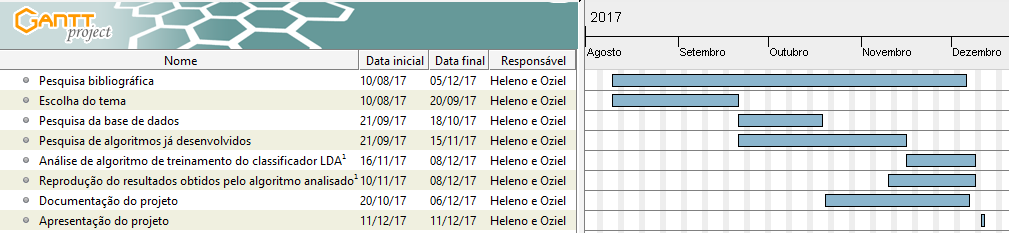
\includegraphics[keepaspectratio=true,scale=0.6]{figuras/cronograma.PNG}
  \caption{Cronograma de atividades já desenvolvidas.}
  \label{cronograma}
\end{figure}


As atividades ainda a serem realizadas neste projeto são apresentadas no cronograma Gantt da Figura \ref{cronograma2}.

\begin{figure}[h]
  \centering
  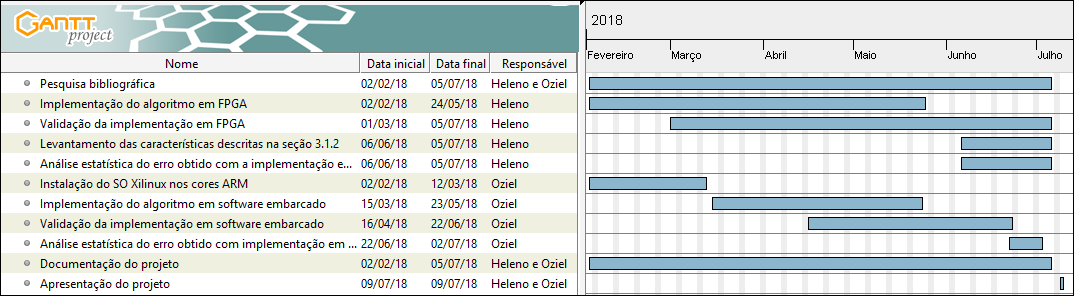
\includegraphics[keepaspectratio=true,scale=0.55]{figuras/cronograma2.PNG}
  \caption{Cronograma de atividades a serem desenvolvidas.}
  \label{cronograma2}
\end{figure}

 \footnote[1]{Algoritmo desenvolvido por \cite{F.Lotte}}
